\documentclass[spanish,xcolor=table,svgnames]{beamer}
\definecolor{mediumpurple4}{rgb}{0.36,0.28,0.55}
%colores coporativos
\definecolor{naranja}{rgb}{0.86,0.42,0.06}
\definecolor{gris}{rgb}{0.41,0.41,0.41}
\definecolor{azul}{rgb}{0.06,0.31,0.55}
\definecolor{rojo}{rgb}{1,0,0}
\usecolortheme[named=azul]{structure}



\mode<presentation>
{

  \usetheme{Copenhagen}
%\useoutertheme{infolines}
  \setbeamercovered{transparent}
  \setbeamertemplate{navigation symbols}{}
}
\usepackage{listings}
\usepackage{color}
\definecolor{gray97}{gray}{.97}
\definecolor{gray75}{gray}{.75}
\definecolor{gray45}{gray}{.45}
\usepackage{listings}
\lstset{ frame=Ltb,
     framerule=0pt,
     aboveskip=0.5cm,
     framextopmargin=3pt,
     framexbottommargin=3pt,
     framexleftmargin=0.4cm,
     framesep=0pt,
     rulesep=.4pt,
     backgroundcolor=\color{gray97},
     rulesepcolor=\color{black},
     %
     stringstyle=\ttfamily,
     showstringspaces = false,
     basicstyle=\small\ttfamily,
     commentstyle=\color{blue},
     keywordstyle=\bfseries,
     %
     numbers=left,
     numbersep=15pt,
     numberstyle=\tiny,
     numberfirstline = false,
     breaklines=true,
   }
 
% minimizar fragmentado de listados
\lstnewenvironment{listing}[1][]
   {\lstset{#1}\pagebreak[0]}{\pagebreak[0]}
 \lstdefinestyle{consola}
   {basicstyle=\scriptsize\bf\ttfamily,
    backgroundcolor=\color{gray75},
   }
\lstdefinestyle{consola}
   {basicstyle=\scriptsize\bf\ttfamily,
    backgroundcolor=\color{gray75},
   }

\lstdefinestyle{XML}
   {language=XML,
   }

\usepackage[spanish]{babel}
\usepackage[utf8x]{inputenc}
\usepackage{charter}
\usepackage[T1]{fontenc}
\usepackage{fancyvrb}
\usepackage{tikz}
%\usepackage{microtype}
\usepackage{xspace}
\usepackage{ctable}
\usepackage{alltt,multicol}

\newcommand{\reduce}{\fontsize{8}{9}\selectfont}
%\usetikzlibrary{chains,positioning,decorations.pathreplacing,fit,scopes}

\title[Título del proyecto]{Título del Proyecto}
\author{Nombre del alumno}
\institute[UCA]{Titulación \\ Universidad de Cádiz}
\date{\today} %poner la fecha

\DefineVerbatimEnvironment{vrbwithcmd}{Verbatim}{commandchars=+(),fontsize=\small}

\begin{document}

\begin{frame}
  \titlepage
  \begin{figure}
	
\includegraphics[height=0.2\textheight]{logo_uca} 
  \end{figure}
\end{frame}

\frame{\frametitle{Índice}\tableofcontents}

%%%%%%%%%%%%%%%%%%%%%%%%%%%%%%%%%
\section{Introducción}
\frame{\frametitle{Introducción}\tableofcontents[currentsection]}

\subsection*{Motivación}
\frame{
\frametitle{Motivación}
  \begin{block}{Motivación del proyecto}

  \end{block}
}

\subsection*{Alcance}
\frame{
     \frametitle{Alcance}
\begin{block}{Información general del proyecto}

\end{block}
}

%%%%%%%%%%%%%%%%%%%%%%%%%%%%%%%%%
\section{Planificación}
\frame{\frametitle{Planificación}\tableofcontents[currentsection]}

\subsection*{Metodología}
\frame{
   \frametitle{Metodología}
\begin{block}{}

\end{block}
}

\subsection*{Calendario}
\frame{
\frametitle{Calendario: ejemplo}
\begin{center}
    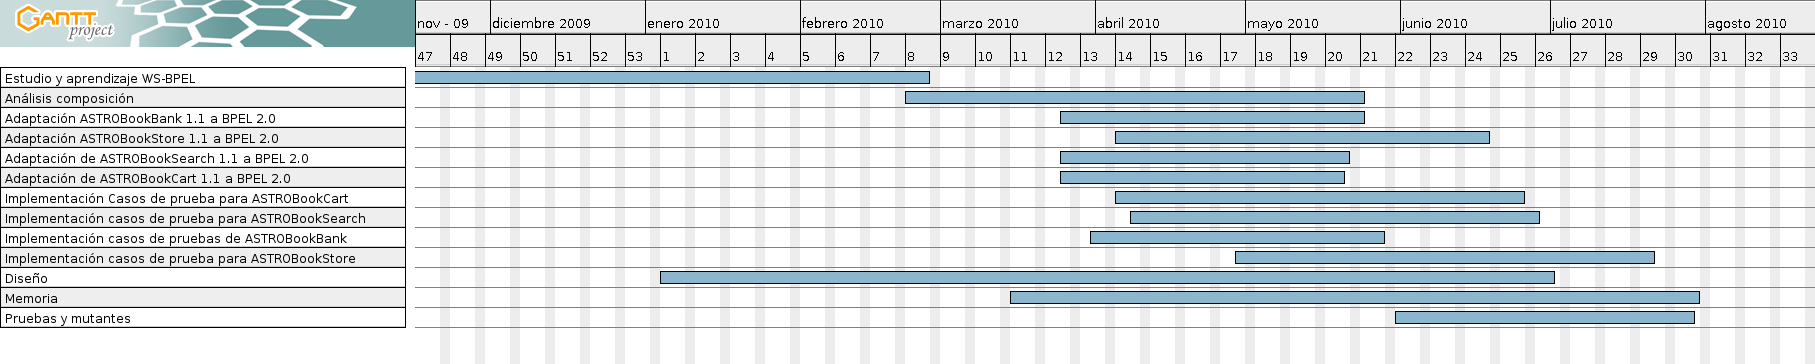
\includegraphics[width=1.0\textwidth]{diagrama_gantt.png}
\end{center}
}

\subsection*{Costes}
\frame{
   \frametitle{Costes}
\begin{block}{Estimación temporal y económica (prevista y real)}

\end{block}
}

\subsection*{Aseguramiento de la Calidad}
\frame{
   \frametitle{Costes}
\begin{block}{}

\end{block}
}

%%%%%%%%%%%%%%%%%%%%%%%%%%%%%%%
\section{Desarrollo del proyecto}
\frame{\frametitle{Desarrollo del proyecto}\tableofcontents[currentsection]}

\subsection*{Requisitos}
\begin{frame}{Requisitos}
  \begin{block}{Requisitos...}

  \end{block}
\end{frame}


\subsection*{Análisis}
\begin{frame}{Análisis}
  \begin{block}{Análisis...}

  \end{block}
\end{frame}

\subsection*{Diseño}
\begin{frame}{Diseño}
  \begin{block}{Diseño...}

  \end{block}
\end{frame}

\subsection*{Implementación}
\begin{frame}{Implementación}
  \begin{block}{Implementación...}

  \end{block}
\end{frame}

\subsection*{Pruebas}
\begin{frame}{Pruebas}
  \begin{block}{Pruebas...}

  \end{block}
\end{frame}

%%%%%%%%%%%%%%%%%%%%%%%%%%%%%%%
\section{Demo}
\frame{\frametitle{Demo}\tableofcontents[currentsection]}

\frame{\frametitle{Demo}
\begin{block}{Presentación del software desarrollado}
\begin{itemize}
\item ....
\item ....
\item ....
\item ....
\end{itemize}
\end{block}
}


%%%%%%%%%%%%%%%%%%%%%%%%%%%%%%%
\section{Conclusiones}
\frame{\frametitle{Conclusiones}\tableofcontents[currentsection]}


\frame{\frametitle{Objetivos alcanzados}
\begin{block}{Los objetivos alcanzados han sido...}
\begin{itemize}
\item Objetivo...
\item ....
\item ....
\item ....
\end{itemize}
\end{block}
}

\frame{\frametitle{Lecciones aprendidas}
\begin{block}{Valoración...}
\begin{itemize}
\item Se ha aprendido...
\item Se ha realizado un buen trabajo de...
\item Conceptos de ...
\end{itemize}
\end{block}
}

\frame{\frametitle{Trabajo futuro}
\begin{block}{Indicar trabajos futuros...}
\begin{itemize}
\item Trabajo futuro 1...
\item ....
\item ....
\item ....
\end{itemize}
\end{block}
}


\frame{\frametitle{Agradecimientos}
\begin{block}{}
- ...
\end{block}
}
\section{Bibliografía}
\frame{\frametitle{Bibliografía}\tableofcontents[currentsection]}
\frame{\frametitle{Bibliografía}

\begin{thebibliography}{10}
\beamertemplatebookbibitems

\bibitem{11}IBM. \emph{Business Process Execution Language for Web Services 1.1}. 2003.
\bibitem{20}IBM-OASIS. \emph{Web Services Business Process Execution Language Version 2.0. OASIS Standard}. abril 2007.
%\bibitem{bibliografia1}....
\end{thebibliography} 
}


\appendix
\frame
{
  \begin{center}
Gracias por su atención\bigskip 

  \end{center}
}
\end{document}
